\section{Multi-Armed Bandit Formulation for Deformable Object Manipulation}

\todoin{Rename this section or the whole chapter}
\todoin{Update main loop to use correct function names per previous chapter}

\begin{algorithm}[ht]
    \caption{MainLoop$(\obstacle, \beta, \lambda)$}
    \begin{algorithmic}[1]
        \State $t \gets 0$
        \State $\RelaxedDistMatrix \gets$ GeodesicDistanceMatrix$(\deformconfig_{relaxed})$
        \State $\modelset \gets$ InitializeModels$(\RelaxedDistMatrix)$
        \State InitialzeBanditAlgorithm()
        \State $\deformconfig(0) \gets$ SensePoints()
        \State $\robotconfig(0) \gets$ SenseRobotConfig()
        \While{true}
            \State $\modelchosen \gets $ SelectArmUsingBanditAlgorithm()
            
            \State $\target \gets$ GetTargets()
            \State $\correspondences \gets$ CalculateCorrespondences$(\deformconfig_t, \target)$
            \State $\deformvel_e, \Pinvweight_e \gets$ FollowNavigationFunction$(\deformconfig_n, \correspondences)$
            \State $\deformvel_s, \Pinvweight_s \gets$ StretchingCorrection$(\RelaxedDistMatrix, \stretchmax, \deformconfig)$
            \State $\deformvel_d, \Pinvweight_d \gets$ CombineTerms$(\deformvel_e, \Pinvweight_e, \deformvel_s, \Pinvweight_s, \stretchweightfactor)$

            \State $\grippervel_d \gets \DeformBackwardFn_m(\deformvel_d, \Pinvweight_d)$
            \State $\grippervel \gets$ ObstacleRepulsion$(\grippervel_d, \obstacle, \obsavoidfactor)$
            
            \State CommandConfiguration$(\gripperconfig(t) + \grippervel)$

            \State $\deformconfig(t + 1) \gets$ SensePoints$()$
            \State $\robotconfig(t + 1) \gets$ SenseRobotConfig$()$
            \State UpdateBanditAlgorithm$()$
            
            \State $t \gets t + 1$
        \EndWhile
    \end{algorithmic}
    \label{alg:mab_mainloop}
\end{algorithm}

\todoin{Move Fig.~\ref{fig:distance} to modelling section.}
\begin{figure}[ht]
    \centering
    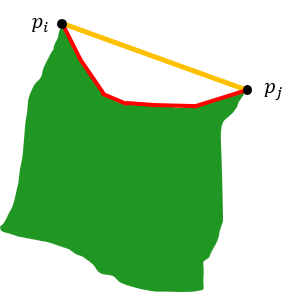
\includegraphics[height=1.5in]{EuclideanVsGeodesic}
    \caption{Euclidean distance measures length of the shortest path between $p_i$ and $p_j$ in $\reals^3$ (gold). Geodesic distance measures the length of the shortest path, constrained to stay within the deformable object (red).}
    \label{fig:distance}
\end{figure}

Our algorithm~(Alg.~\ref{alg:mab_mainloop}) can be broken down into four major sections and an initialization block. In the initialization block we pre-compute the geodesic distance (see Fig.~\ref{fig:distance}) between every pair of points in $\deformconfig$ when the deformable object is in its ``natural'' or ``relaxed'' state and store the result in $\RelaxedDistMatrix$. These distances are used to construct the deformation models~(Sec.~\ref{sec:jacobian_models}), as well as to avoid overstretching the object (Sec.~\ref{sec:stretching_avoidance_old}).
At each iteration we: 
\begin{enumerate}
    \item pick a model to use to achieve the desired direction~(Sec.~\ref{sec:bandit_algorithms}); 
    \item compute the task-defined desired direction to move the deformable object~(Sec.~\ref{sec:reducing_error}); 
    \item generate a velocity command using the chosen model~(Sec.~\ref{sec:stretching_avoidance_controller}); 
    \item modify the command to avoid obstacles~(Sec.~\ref{sec:stretching_avoidance_controller});
    \item update bandit algorithm parameters~(Sec.~\ref{sec:bandit_algorithms}).
\end{enumerate}


